\documentclass[]{article}

\usepackage{longtable}
\usepackage{caption}

\usepackage{amsmath}
\usepackage{makeidx}
\usepackage{lscape}
\usepackage{graphicx}
	 
%opening
\title{Report on panel model results}
\author{Vicente López Díaz}
\makeindex

\begin{document}

\maketitle

\begin{abstract}
These notes relate panel data models used for data with two levels (city and brand) additional to time.
\end{abstract}

The objective is to relate the models that can describe the data. There are several usual features to consider in a model with panel data, for example, changes on parameters for time or individual. Also, specification on error term is relevant for interpretation.

\section{Data plots}
Here is a summary of the data available for the analysis. 

Figure 1 presents the initial data points used for the analysis.

To decide which brands to include, I considered the number of observations on the period previous to the tax implementation, the tax started in january 2020, I made an exploratory analysis on the december 2019 data. This would ease the estimation, brands with few observations would have difficulties to calculate most estimates. Data for brands with few observations can be analyzed after defining a criteria to form brand groups.

\begin{figure}
\begin{center}
	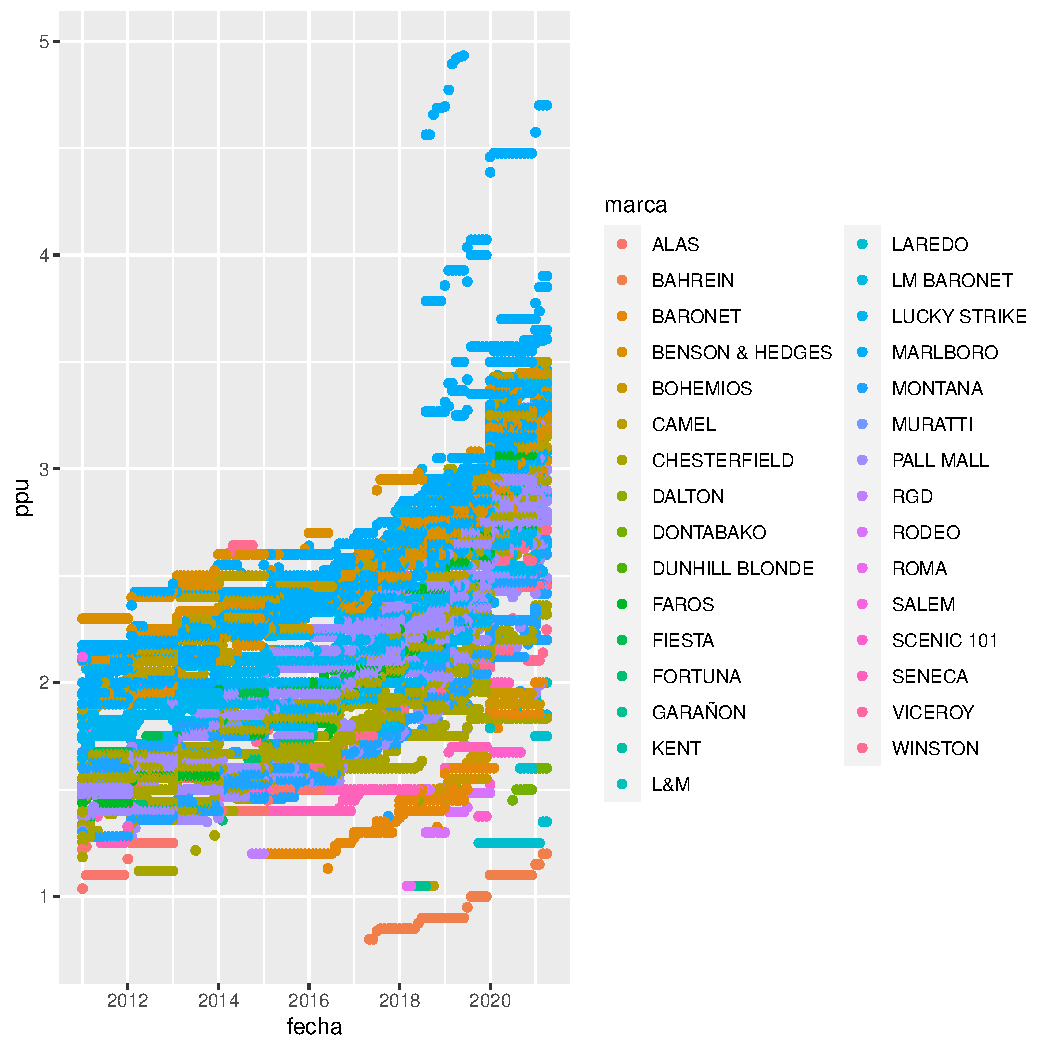
\includegraphics[width=\textwidth]{df_review_ppu_marcas.pdf} 
\end{center}
 \caption{All brands average price per unit}
\end{figure}

Figure 2 only considers the 7 most frequent brands. The graph provides some guidance on what to consider for the proposed descriptive model.  In particular, there is clear trend over time and there are price adjustments in almost every january. 
Results only consider data for the 7 brands. Brand labels are alphabetic, as shown in the graph: 1, Benson; 2, Camel; 3, Chesterfield; 4, Lucky; 5, Marlboro; 6, Montana; 7, Pall Mall.

\begin{figure}
\begin{center}
		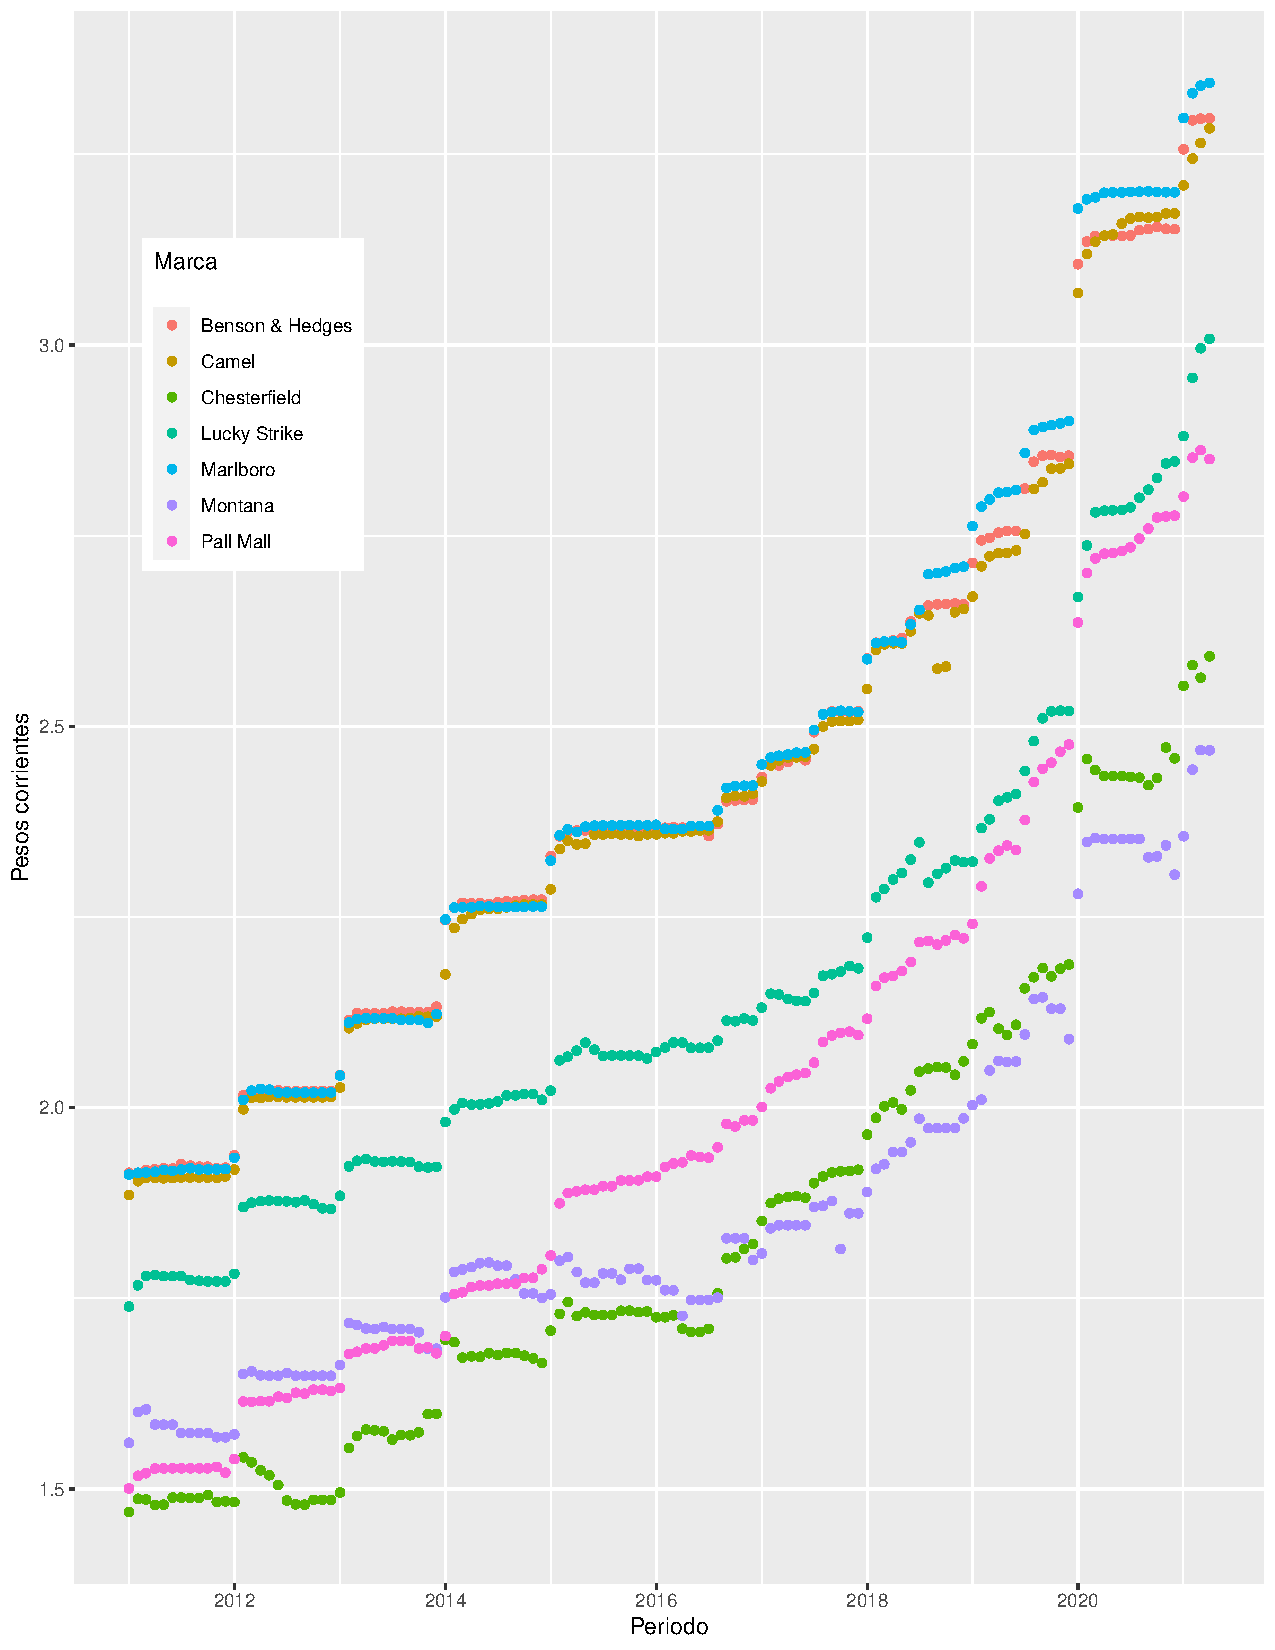
\includegraphics[width=\textwidth]{prin7_prom_ppu_marcas.pdf} 
\end{center}
 \caption{Seven brands average price per unit}
\end{figure}

Except for prices of other products, there are no other potential regressors to consider at the same level of the data.

\section{Dummies for each level: city, brand, time}
Estimations in this section use areg, it imposes fixed effects. Using  this method there is one category with parameters "absorbed", which are not estimated as a result of the procedure.

Specification with indicators for city, brand and trend time, with the same tax effect on all the brands.

\begin{equation*} 
y_{ctm}  = \alpha_{i}^{*} + \gamma_{m}^{*} + \lambda*trend + \beta_{0}^{'}jan + \beta_{1}^{'}tax2020 + \beta_{1}^{'}tax2021 + u_{ctm}
;   \tag{2.1}
\end{equation*}
$c  = 1,\ldots,N;  t=1,\ldots,T; m=1,\ldots,M. $

Specification with indicators for city, brand and trend time, with interacted effect for each brand.

\begin{equation*} 
	y_{ctm}  = \alpha_{i}^{*} + \gamma_{m}^{*} + \lambda*trend + \beta_{0}^{'}jan + \beta_{1m}^{'}tax2020 + \beta_{2m}^{'}tax2021 + u_{itm}
	;   \tag{2.2}
\end{equation*}
$c  = 1,\ldots,N;  t=1,\ldots,T; m=1,\ldots,M. $

Dummy variables for time month and year, with same tax for all brands.
\begin{equation*} 
	y_{ctm}  = \alpha_{i}^{*} + \gamma_{m}^{*} + month + year + \beta_{0}^{'}jan + \beta_{1}^{'}tax2020 + \beta_{2}^{'}tax2021 + u_{itm}
	;   \tag{2.3}
\end{equation*}

Dummy variables for time month and year, with different tax for each brand.

\begin{equation*} 
	y_{ctm}  = \alpha_{i}^{*} + \gamma_{m}^{*} + month + year + \beta_{0}^{'}jan + \beta_{1m}^{'}tax2020 + \beta_{2m}^{'}tax2021 + u_{itm}
	;   \tag{2.4}
\end{equation*}

The columns 1 and 3 consider the same effect for each brand (2.1) and (2.3), the columns 2 and 4 estimate a different effect for each brand (2.2) and (2.4). The columns 1 and 2 consider a time trend, columns 3 and 4 use a combination of dummy variables for year and month.

\begin{longtable}{lcccc} 
\caption{Fixed Effects for city and brand combination}\label{tab:1}\\	
	\hline
 & (1) & (2) & (3) & (4) \\
%\begin{tabular}{lcccc} \hline
%	& (1) & (2) & (3) & (4) \\
VARIABLES & ppu & ppu & ppu & ppu \\ \hline
 &  &  &  &  \\
jan20 & 0.209*** & 0.238*** & -0.017* & 0.012 \\
& (0.011) & (0.024) & (0.009) & (0.018) \\
jan21 & 0.242*** & 0.285*** & -0.011 & 0.032* \\
& (0.011) & (0.024) & (0.010) & (0.019) \\
jan & -0.024*** & -0.024*** & -0.069*** & -0.069*** \\
& (0.004) & (0.004) & (0.004) & (0.004) \\
jan20\#2.marca &  & -0.007 &  & -0.012 \\
 &  & (0.042) &  & (0.032) \\
jan20\#3.marca &  & -0.111** &  & -0.112*** \\
 &  & (0.043) &  & (0.033) \\
jan20\#4.marca &  & -0.147*** &  & -0.150*** \\
 &  & (0.039) &  & (0.030) \\
jan20\#5.marca &  & 0.052 &  & 0.051** \\
 &  & (0.032) &  & (0.024) \\
jan20\#6.marca &  & -0.239*** &  & -0.235*** \\
 &  & (0.062) &  & (0.048) \\
jan20\#7.marca &  & -0.028 &  & -0.024 \\
 &  & (0.034) &  & (0.026) \\
jan21\#2.marca &  & -0.035 &  & -0.040 \\
 &  & (0.040) &  & (0.031) \\
jan21\#3.marca &  & -0.116** &  & -0.118*** \\
 &  & (0.046) &  & (0.035) \\
jan21\#4.marca &  & -0.132*** &  & -0.134*** \\
 &  & (0.038) &  & (0.029) \\
jan21\#5.marca &  & 0.022 &  & 0.021 \\
 &  & (0.032) &  & (0.024) \\
jan21\#6.marca &  & -0.361*** &  & -0.357*** \\
 &  & (0.063) &  & (0.048) \\
jan21\#7.marca &  & -0.036 &  & -0.031 \\
 &  & (0.034) &  & (0.026) \\
2.marca & -0.012*** & -0.011*** & -0.006** & -0.006** \\
& (0.003) & (0.003) & (0.003) & (0.003) \\
3.marca & -0.595*** & -0.593*** & -0.592*** & -0.591*** \\
& (0.004) & (0.004) & (0.003) & (0.003) \\
4.marca & -0.270*** & -0.268*** & -0.268*** & -0.266*** \\
& (0.003) & (0.003) & (0.003) & (0.003) \\
5.marca & 0.011*** & 0.010*** & 0.011*** & 0.010*** \\
& (0.003) & (0.003) & (0.002) & (0.002) \\
6.marca & -0.524*** & -0.521*** & -0.527*** & -0.524*** \\
& (0.005) & (0.005) & (0.004) & (0.004) \\
7.marca & -0.435*** & -0.435*** & -0.441*** & -0.440*** \\
& (0.003) & (0.003) & (0.002) & (0.002) \\
ym & 0.009*** & 0.009*** &  &  \\
 & (0.000) & (0.000) &  &  \\
Constant & -3.925*** & -3.926*** & 1.991*** & 1.990*** \\
 & (0.018) & (0.018) & (0.004) & (0.004) \\
 &  &  &  &  \\
Observations & 24,010 & 24,010 & 24,010 & 24,010 \\
 R-squared & 0.897 & 0.897 & 0.940 & 0.940 \\ \hline
\multicolumn{5}{c}{ Standard errors in parentheses} \\
\multicolumn{5}{c}{ *** p$<$0.01, ** p$<$0.05, * p$<$0.1} \\
%\end{tabular}
\end{longtable}

%\begin{tabular}{lcccc} \hline
 & (1) & (2) & (3) & (4) \\
VARIABLES & ppu & ppu & ppu & ppu \\ \hline
 &  &  &  &  \\
m1 & -0.023*** & -0.023*** & -0.071*** & -0.071*** \\
 & (0.003) & (0.003) & (0.003) & (0.003) \\
1.m1\_20 &  & 0.248*** &  & 0.017 \\
 &  & (0.021) &  & (0.016) \\
2.marca & -0.010*** & -0.010*** & -0.005* & -0.005* \\
 & (0.003) & (0.003) & (0.003) & (0.003) \\
3.marca & -0.593*** & -0.593*** & -0.591*** & -0.590*** \\
 & (0.003) & (0.003) & (0.003) & (0.003) \\
4.marca & -0.270*** & -0.269*** & -0.268*** & -0.267*** \\
 & (0.003) & (0.003) & (0.003) & (0.003) \\
5.marca & 0.012*** & 0.011*** & 0.012*** & 0.012*** \\
 & (0.003) & (0.003) & (0.002) & (0.002) \\
6.marca & -0.528*** & -0.526*** & -0.532*** & -0.530*** \\
 & (0.005) & (0.005) & (0.004) & (0.004) \\
7.marca & -0.431*** & -0.431*** & -0.436*** & -0.436*** \\
 & (0.003) & (0.003) & (0.002) & (0.002) \\
0b.m1\_20\#1b.marca &  & 0.000 &  & 0.000 \\
 &  & (0.000) &  & (0.000) \\
0b.m1\_20\#2o.marca &  & 0.000 &  & 0.000 \\
 &  & (0.000) &  & (0.000) \\
0b.m1\_20\#3o.marca &  & 0.000 &  & 0.000 \\
 &  & (0.000) &  & (0.000) \\
0b.m1\_20\#4o.marca &  & 0.000 &  & 0.000 \\
 &  & (0.000) &  & (0.000) \\
0b.m1\_20\#5o.marca &  & 0.000 &  & 0.000 \\
 &  & (0.000) &  & (0.000) \\
0b.m1\_20\#6o.marca &  & 0.000 &  & 0.000 \\
 &  & (0.000) &  & (0.000) \\
0b.m1\_20\#7o.marca &  & 0.000 &  & 0.000 \\
 &  & (0.000) &  & (0.000) \\
1o.m1\_20\#1b.marca &  & 0.000 &  & 0.000 \\
 &  & (0.000) &  & (0.000) \\
1.m1\_20\#2.marca &  & -0.007 &  & -0.014 \\
 &  & (0.037) &  & (0.029) \\
1.m1\_20\#3.marca &  & -0.107*** &  & -0.111*** \\
 &  & (0.039) &  & (0.031) \\
1.m1\_20\#4.marca &  & -0.143*** &  & -0.151*** \\
 &  & (0.036) &  & (0.028) \\
1.m1\_20\#5.marca &  & 0.055* &  & 0.053** \\
 &  & (0.028) &  & (0.022) \\
1.m1\_20\#6.marca &  & -0.271*** &  & -0.264*** \\
 &  & (0.053) &  & (0.041) \\
1.m1\_20\#7.marca &  & -0.031 &  & -0.027 \\
 &  & (0.030) &  & (0.023) \\
ym & 0.009*** & 0.009*** &  &  \\
 & (0.000) & (0.000) &  &  \\
m1\_20 & 0.220*** &  & -0.013 &  \\
 & (0.010) &  & (0.008) &  \\
 &  &  &  &  \\
Observations & 24,276 & 24,276 & 24,276 & 24,276 \\
 R-squared & 0.897 & 0.898 & 0.938 & 0.938 \\ \hline
\multicolumn{5}{c}{ Standard errors in parentheses} \\
\multicolumn{5}{c}{ *** p$<$0.01, ** p$<$0.05, * p$<$0.1} \\
\end{tabular}


Results only consider data for the 7 brands. In the results they have a number as label assigned in alphabetic order, the same shown in the graph: 1, Benson; 2, Camel; 3, Chesterfield; 4, Lucky; 5, Marlboro; 6, Montana; 7, Pall Mall.

Although the model with dummy time variables fits the data better, R-squared, for ease of analysis of the tax effect the model with trend will be used subsequently. Because the tax effect in the last models is spread in the combination of year and month, together with the explicit coefficients for january 2020 and january 2021.  

\subsection{Comparisons by segment}
This section separates the previous estimation of interactions by brand type or segment.

Results by brand type: premium, columns 1 and 2; medium, columns 3 and 4; low, columns 5 and 6.
The omitted identifier corresponds to the reference brand.

%\begin{landscape}
	\begin{longtable}{lcccccc} 
	\caption{Fixed Effects by brand type}\label{tab:2}\\	
	\hline
%\begin{tabular}{lcccccc} \hline
 & (1) & (2) & (3) & (4) & (5) & (6) \\
VARIABLES & ppu & ppu & ppu & ppu & ppu & ppu \\ \hline
 &  &  &  &  &  &  \\
jan20 & 0.219*** & 0.198*** & 0.182*** & 0.119*** & 0.191*** & 0.225*** \\
& (0.012) & (0.019) & (0.021) & (0.033) & (0.034) & (0.040) \\
jan21 & 0.238*** & 0.235*** & 0.235*** & 0.188*** & 0.231*** & 0.310*** \\
& (0.012) & (0.019) & (0.021) & (0.033) & (0.036) & (0.042) \\
jan & -0.018*** & -0.018*** & -0.040*** & -0.040*** & -0.013 & -0.013 \\
& (0.004) & (0.004) & (0.007) & (0.007) & (0.009) & (0.009) \\
jan20\#2.marca &  & -0.009 &  &  &  &  \\
 &  & (0.032) &  &  &  &  \\
jan20\#5.marca &  & 0.051** &  &  &  &  \\
&  & (0.025) &  &  &  &  \\
jan20\#6.marca &  &  &  &  &  & -0.119* \\
&  &  &  &  &  & (0.072) \\
jan20\#7.marca &  &  &  & 0.102** &  &  \\
&  &  &  & (0.041) &  &  \\
jan21\#2.marca &  & -0.037 &  &  &  &  \\
 &  & (0.031) &  &  &  &  \\
jan21\#5.marca &  & 0.022 &  &  &  &  \\
 &  & (0.025) &  &  &  &  \\
jan21\#6.marca &  &  &  &  &  & -0.252*** \\
&  &  &  &  &  & (0.073) \\
jan21\#7.marca &  &  &  & 0.076* &  &  \\
&  &  &  & (0.040) &  &  \\
2.marca & -0.008*** & -0.007*** &  &  &  &  \\
& (0.003) & (0.003) &  &  &  &  \\
5.marca & 0.008*** & 0.007*** &  &  &  &  \\
& (0.002) & (0.002) &  &  &  &  \\
6.marca &  &  &  &  & 0.101*** & 0.102*** \\
&  &  &  &  & (0.007) & (0.007) \\
7.marca &  &  & -0.165*** & -0.166*** &  &  \\
&  &  & (0.004) & (0.004) &  &  \\
ym & 0.010*** & 0.010*** & 0.009*** & 0.009*** & 0.007*** & 0.007*** \\
 & (0.000) & (0.000) & (0.000) & (0.000) & (0.000) & (0.000) \\
Constant & -4.429*** & -4.429*** & -4.040*** & -4.041*** & -2.892*** & -2.895*** \\
 & (0.019) & (0.019) & (0.037) & (0.037) & (0.051) & (0.051) \\
 &  &  &  &  &  &  \\
Observations & 13,396 & 13,396 & 6,700 & 6,700 & 3,914 & 3,914 \\
 R-squared & 0.917 & 0.918 & 0.846 & 0.846 & 0.760 & 0.761 \\ \hline
\multicolumn{7}{c}{ Standard errors in parentheses} \\
\multicolumn{7}{c}{ *** p$<$0.01, ** p$<$0.05, * p$<$0.1} \\
%\end{tabular}
\end{longtable}

%\begin{tabular}{lccc} \hline
 & (1) & (2) & (3) \\
VARIABLES & ppu & ppu & ppu \\ \hline
 &  &  &  \\
m1 & -0.018*** & -0.039*** & -0.012 \\
 & (0.004) & (0.007) & (0.008) \\
m1\_20 & 0.233*** & 0.195*** & 0.194*** \\
 & (0.011) & (0.019) & (0.029) \\
ym & 0.010*** & 0.009*** & 0.007*** \\
 & (0.000) & (0.000) & (0.000) \\
 &  &  &  \\
Observations & 13,598 & 6,737 & 3,941 \\
 R-squared & 0.916 & 0.844 & 0.773 \\ \hline
\multicolumn{4}{c}{ Standard errors in parentheses} \\
\multicolumn{4}{c}{ *** p$<$0.01, ** p$<$0.05, * p$<$0.1} \\
\end{tabular}

%\end{landscape}

Brand labels are alphabetic: 1, Benson; 2, Camel; 3, Chesterfield; 4, Lucky; 5, Marlboro; 6, Montana; 7, Pall Mall.

Table \ref{tab:Fareg} shows results to tests coefficient equality between brands. The first two rows correspond to the complete sample (Table 1, columns 1 and 2). Rows third and fourth test for difference in premium brands (Table 2, columns 1 and 2). Rows fifth and sixth test for difference in medium brands (Table 2, column 3 and 4). Rows seventh and eighth test for difference in lower priced brands (Table 2, column 5 and 6). Columns 1 to 3 indicate the parameters and result for the the test of fixed effects or individual effects by brand. Columns 4 to 6 show the values to test for the equality of the effect by brand of the tax in 2020. Columns 7 to 9 show the values and test result for the equality of the effect by brand of the tax in 2021.


\begin{landscape}
	\begin{table}[ht]
		\centering
		% To place a caption above a table
		\caption{F tests for equality of coefficients \label{tab:Fareg}} 
	%\begin{table}[ht] 
\begin{tabular}{lccccccccc} 
	\hline
	& (1) & (2) & (3) & (4) & (5) & (6)  & (7) & (8) & (9) \\
	&\multicolumn{3}{c}{Equality of Intercept} &\multicolumn{3}{c}{Equality of Tax 2020} &\multicolumn{3}{c}{Equality of Tax 2021}\\
	Equation&Numerator&Denominator&F&Numerator&Denominator&F&Numerator&Denominator&F\\
	(2.1)&6&23954&10163.44\\
	(2.2)&6&23942&10006.08&6&23942&8.15&6&23942&9.14\\
	(2.1)&2&13344&19.05\\
	(2.2)&2&13340&16.81&2&13340&2.89&2&13340&1.88\\
	(2.1)&1&6649&1604.66\\
	(2.2)&1&6647&1613.81&1&6647&6.09&1&6647&3.52\\
	(2.1)&1&3867&187\\
	(2.2)&1&3865&193.13&1&3865&2.74&1&3865&11.8\\
	\hline
	\multicolumn{10}{c}{ All tests are significant at 1 percent level} \\

%\end{table}
\end{tabular}

	%\caption{Caption below table.}

	\end{table}
\end{landscape}

\section{Constant Parameters over time}
This section presents estimations using xtreg. The first subsection presents static estimations, the second subsection contains dynamic estimates.

\subsection{Static models}
The first model includes the effect of the price change in every january, january 2020 and january 2021 and trend.

\begin{equation*} 
	y_{it}  = \alpha_{i}^{*} + \gamma_{m}^{*} + \lambda*trend + \beta_{0}^{'}jan + \beta_{1}^{'}tax2020 + \beta_{1}^{'}tax2021 + u_{it}
	;   \tag{4.1}
\end{equation*}
$c  = 1,\ldots,N;  t=1,\ldots,T; m=1,\ldots,M. $

The second model includes interactions for the effect of the price change in january 2020 and january 2021, for different brand-types.

\begin{equation*} 
	y_{it}  = \alpha_{i}^{*} + \gamma_{m}^{*} + \lambda*trend + \beta_{0}^{'}jan + \beta_{1m}^{'}tax2020 + \beta_{2m}^{'}tax2021 + u_{it}
	;   \tag{4.2}
\end{equation*}
$i  = 1,\ldots,N;  t=1,\ldots,T; m=1,\ldots,M. $

Because there are many omitted variables captured in the individual effects, there is the question of the relevance of them as fixed or random.

The result of the Hausman test for fixed effects does not rule out the non systematic difference in coefficients, this is in favour of the random effects model: Chi2(4) =  0.60,
$Prob \geq chi2 =    0.9628$

Similarly the Breusch-Pagan test for random effects does rule out the alternative of OLS : chibar2(01) =  7.5e+05,
$Prob \geq chibar2 =    0.0000$

The test of unit root, using the Fischer type estimation from Choi (2001): 
Inverse chi-squared(500) = 1112.8056 , $Prob \geq chi2 =    0.0000$, does not rule out the presence of unit root for any panel (defined as a combination of city and brand), except for the model that includes a drift. The result suggests to consider different trends for each brand or city, there is an estimation by brand to test for unit roots by specifications of the panel.

Next are the results from the complete sample,
columns (1,2,4,5) are estimated using random effects. The third column presents fixed individual effects estimates, since the estimates by brand (presented next) suggest that most brands have fixed effects for city.

Column (1) corresponds to the equation (4.1), column (4) restricts the estimation in column (1) to zero trend. Column (2) corresponds to equation (4.2) column (4)  restricts the estimation in column (4) to zero trend. Column (3) corresponds to column (2) estimated using fixed effects.

%\begin{tabular}{lccccc} 
\begin{longtable}{lccccc}
	\caption{Fixed Effects for brand and city by brand type}\label{tab:xt1}\\	
	
	\hline
 & (1) & (2) & (3) & (4) & (5) \\
VARIABLES & ppu & ppu & ppu & ppu & ppu \\ \hline
 &  &  &  &  &  \\
jan20 & 0.202*** & 0.230*** & 0.230*** & -0.015** & 0.012 \\
 & (0.010) & (0.021) & (0.021) & (0.007) & (0.015) \\
jan21 & 0.232*** & 0.276*** & 0.275*** & -0.012 & 0.027* \\
 & (0.010) & (0.021) & (0.021) & (0.008) & (0.016) \\
jan & -0.023*** & -0.023*** & -0.023*** & -0.070*** & -0.070*** \\
& (0.003) & (0.003) & (0.003) & (0.003) & (0.003) \\
2.marca\#jan20 &  & -0.012 & -0.011 &  & -0.011 \\
&  & (0.037) & (0.037) &  & (0.026) \\
3.marca\#jan20 &  & -0.109*** & -0.108*** &  & -0.103*** \\
&  & (0.039) & (0.039) &  & (0.027) \\
4.marca\#jan20 &  & -0.125*** & -0.124*** &  & -0.129*** \\
&  & (0.034) & (0.034) &  & (0.024) \\
5.marca\#jan20 &  & 0.056** & 0.056** &  & 0.052*** \\
&  & (0.028) & (0.028) &  & (0.020) \\
6.marca\#jan20 &  & -0.194*** & -0.191*** &  & -0.195*** \\
&  & (0.056) & (0.056) &  & (0.039) \\
7.marca\#jan20 &  & -0.052* & -0.053* &  & -0.040* \\
&  & (0.030) & (0.030) &  & (0.021) \\
2.marca\#jan21 &  & -0.047 & -0.051 &  & -0.039 \\
 &  & (0.036) & (0.036) &  & (0.025) \\
3.marca\#jan21 &  & -0.101** & -0.101** &  & -0.100*** \\
 &  & (0.041) & (0.041) &  & (0.029) \\
4.marca\#jan21 &  & -0.117*** & -0.118*** &  & -0.113*** \\
 &  & (0.034) & (0.034) &  & (0.024) \\
5.marca\#jan21 &  & 0.027 & 0.027 &  & 0.022 \\
 &  & (0.028) & (0.028) &  & (0.020) \\
6.marca\#jan21 &  & -0.364*** & -0.364*** &  & -0.360*** \\
 &  & (0.056) & (0.056) &  & (0.039) \\
7.marca\#jan21 &  & -0.053* & -0.051* &  & -0.033 \\
 &  & (0.030) & (0.030) &  & (0.021) \\
2.marca & -0.013 & -0.013 &  & -0.009 & -0.008 \\
& (0.024) & (0.022) &  & (0.018) & (0.017) \\
3.marca & -0.605*** & -0.604*** &  & -0.603*** & -0.602*** \\
& (0.024) & (0.022) &  & (0.018) & (0.017) \\
4.marca & -0.274*** & -0.272*** &  & -0.269*** & -0.268*** \\
& (0.024) & (0.021) &  & (0.017) & (0.017) \\
5.marca & 0.004 & 0.004 &  & 0.007 & 0.007 \\
& (0.022) & (0.020) &  & (0.016) & (0.016) \\
6.marca & -0.502*** & -0.500*** &  & -0.505*** & -0.503*** \\
& (0.028) & (0.026) &  & (0.021) & (0.020) \\
7.marca & -0.426*** & -0.425*** &  & -0.443*** & -0.442*** \\
& (0.023) & (0.021) &  & (0.017) & (0.017) \\
ym & 0.009*** & 0.009*** & 0.009*** &  &  \\
& (0.000) & (0.000) & (0.000) &  &  \\
Constant & -3.940*** & -3.940*** & -4.137*** & 1.989*** & 1.989*** \\
 & (0.023) & (0.022) & (0.017) & (0.012) & (0.012) \\
 &  &  &  &  &  \\
Observations & 23,926 & 23,926 & 23,926 & 23,926 & 23,926 \\
Number of gr\_marca\_ciudad & 263 & 263 & 263 & 263 & 263 \\
 R-squared &  &  & 0.866 &  &  \\ \hline
\multicolumn{6}{c}{ Standard errors in parentheses} \\
\multicolumn{6}{c}{ *** p$<$0.01, ** p$<$0.05, * p$<$0.1} \\
%\end{tabular}
\end{longtable}


Next table present the results by brand type: premium, columns 1 and 2; medium, columns 3 and 4; low, columns 5 and 6. The omitted identifier corresponds to the reference brand. Columns (1,3,5) correspond to the equation (4.1), columns (2,4,6) correspond to equation (4.2). 

\begin{longtable}{lcccccc} 
%\begin{tabular}{lcccccc} 
	\caption{Fixed Effects/Random Effects for brand and city by brand type}\label{tab:xt2}\\	
	\hline
 & (1) & (2) & (3) & (4) & (5) & (6) \\
VARIABLES & ppu & ppu & ppu & ppu & ppu & ppu \\ \hline
 &  &  &  &  &  &  \\
4.marca &  &  & -4.013*** & 0.150*** &  &  \\
 &  &  & (0.041) & (0.028) &  &  \\
1.m1\_20 &  & 0.196*** &  & 0.132*** &  & 0.212*** \\
 &  & (0.018) &  & (0.030) &  & (0.037) \\
1.m1\_20\#7.marca &  &  &  & 0.071* &  &  \\
 &  &  &  & (0.037) &  &  \\
1.m1\_21 &  & 0.233*** &  & 0.251*** &  & 0.295*** \\
 &  & (0.018) &  & (0.024) &  & (0.040) \\
1.m1\_21\#4.marca &  &  &  & -0.062* &  &  \\
 &  &  &  & (0.037) &  &  \\
m1 & -0.018*** & -0.018*** & -0.039*** & -0.039*** & -0.012 & -0.012 \\
 & (0.004) & (0.004) & (0.006) & (0.006) & (0.008) & (0.008) \\
ym & 0.010*** & 0.010*** & 0.009*** & 0.009*** & 0.007*** & 0.007*** \\
 & (0.000) & (0.000) & (0.000) & (0.000) & (0.000) & (0.000) \\
1.m1\_20\#2.marca &  & -0.012 &  &  &  &  \\
 &  & (0.031) &  &  &  &  \\
1.m1\_20\#5.marca &  & 0.053** &  &  &  &  \\
 &  & (0.024) &  &  &  &  \\
1.m1\_21\#2.marca &  & -0.049 &  &  &  &  \\
 &  & (0.030) &  &  &  &  \\
1.m1\_21\#5.marca &  & 0.024 &  &  &  &  \\
 &  & (0.024) &  &  &  &  \\
m1\_20 & 0.218*** &  & 0.176*** &  & 0.190*** &  \\
 & (0.011) &  & (0.019) &  & (0.032) &  \\
m1\_21 & 0.235*** &  & 0.228*** &  & 0.217*** &  \\
 & (0.011) &  & (0.019) &  & (0.034) &  \\
7.marca &  &  & -4.162*** &  &  &  \\
 &  &  & (0.041) &  &  &  \\
1.m1\_20\#6.marca &  &  &  &  &  & -0.078 \\
 &  &  &  &  &  & (0.068) \\
1.m1\_21\#6.marca &  &  &  &  &  & -0.245*** \\
 &  &  &  &  &  & (0.069) \\
Constant & -4.417*** & -4.416*** &  & -4.164*** & -2.961*** & -2.963*** \\
 & (0.019) & (0.019) &  & (0.041) & (0.050) & (0.049) \\
 &  &  &  &  &  &  \\
Observations & 13,396 & 13,396 & 6,620 & 6,620 & 3,910 & 3,910 \\
R-squared & 0.916 & 0.916 &  &  & 0.720 & 0.721 \\
 Number of gr\_marca\_ciudad & 126 & 126 & 80 & 80 & 57 & 57 \\ \hline
\multicolumn{7}{c}{ Standard errors in parentheses} \\
\multicolumn{7}{c}{ *** p$<$0.01, ** p$<$0.05, * p$<$0.1} \\
%\end{tabular}
\end{longtable}


By brand type, for premium(1) and low(3) brand types the Hausman test (see  Table \ref{tab:AppHausmanStatic}) rejects the alternative of random effects in favour of fixed individual effects. The test for type 1 and 3 are Chi2(4) =  0.60,
$Prob \geq chi2 =    0.9628$ and Chi2(4) =  0.60,
$Prob \geq chi2 =    0.9628$, respectively. 

Similarly the Breusch-Pagan test for random effects does rule out the alternative of OLS : chibar2(01) =  7.5e+05,
$Prob \geq chibar2 =    0.0000$

The test of unit root, using the Fischer type estimation from Choi (2001): 
Inverse chi-squared(500) = 1112.8056 , $Prob \geq chi2 =    0.0000$, does not rule out the presence of unit root for any panel (defined as a combination of city and brand), except for the model that includes a drift. The result suggests to consider different trends for each brand or city, there is an estimation by brand to test for unit roots by specifications of the panel. See Table \ref{tab:AppUnitRoots}.

The next table presents F or Chi-squared tests for equality of coeficients, F corresponds to models by fixed effects, Chi-squared corresponds to models estimated by random effects.

The distribution is the same used in Table \ref{tab:Fareg}, first two rows correspond to the complete sample. Rows third and fourth test for difference in premium brands. Rows fifth and sixth test for difference in medium brands. Rows seventh and eighth test for difference in lower priced brands.
Columns 1 to 3 indicate the parameters and result for the the test of fixed effects or individual effects by brand. Columns 4 to 6 show the values to test for the equality of the effect by brand of the tax in 2020. Columns 7 to 9 show the values and test result for the equality of the effect by brand of the tax in 2021.

Except for the effect of the tax in 2020 for lower priced brands, based on these F tests, the prefered model includes interactions by brand.

\begin{landscape}
	\begin{table}[ht]
		\centering
		% To place a caption above a table
		\caption{F tests for equality of coefficients \label{tab:Fxtreg}} 
	\begin{tabular}{lccccccccc} \hline
& (1) & (2) & (3) & (4) & (5) & (6)  & (7) & (8) & (9) \\
&\multicolumn{3}{c}{Equality of Intercept} &\multicolumn{3}{c}{Equality of Tax 2020} &\multicolumn{3}{c}{Equality of Tax 2021}\\
Equation&Num/gl-chi2&Den&F/Chi2&Num/gl-chi2&Den&F/Chi2&Num/gl-chi2&Den&F/Chi2\\
(4.1)&6&&1287.39***\\
(4.2)&6&&1547.03***&6&&51.86***&6&&67.31***\\
(4.1)&125&13266&22.32***\\
(4.2)&125&13262&22.32***&2&13262&3.51**&2&13262&3.08***\\
(4.1)&2&&11224.48***\\
(4.2)&1&&28.63***&1&&3.62*&1&&2.85*\\
(4.1)&56&3849&41.93***\\
(4.2)&56&3847&42.17***&1&3847&1.32&1&3847&12.43*\\
\hline
\multicolumn{10}{c}{ *** p$<$0.01, ** p$<$0.05, * p$<$0.1} \\
\end{tabular}

	\end{table}
\end{landscape}
%\begin{landscape}
%	\begin{tabular}{lccccccccc} \hline
& (1) & (2) & (3) & (4) & (5) & (6)  & (7) & (8) & (9) \\
&\multicolumn{3}{c}{Equality of Intercept} &\multicolumn{3}{c}{Equality of Tax 2020} &\multicolumn{3}{c}{Equality of Tax 2021}\\
Equation&Num/gl-chi2&Den&F/Chi2&Num/gl-chi2&Den&F/Chi2&Num/gl-chi2&Den&F/Chi2\\
(4.1)&6&&1287.39***\\
(4.2)&6&&1547.03***&6&&51.86***&6&&67.31***\\
(4.1)&125&13266&22.32***\\
(4.2)&125&13262&22.32***&2&13262&3.51**&2&13262&3.08***\\
(4.1)&2&&11224.48***\\
(4.2)&1&&28.63***&1&&3.62*&1&&2.85*\\
(4.1)&56&3849&41.93***\\
(4.2)&56&3847&42.17***&1&3847&1.32&1&3847&12.43*\\
\hline
\multicolumn{10}{c}{ *** p$<$0.01, ** p$<$0.05, * p$<$0.1} \\
\end{tabular}

%\end{landscape}

The next table presents the static results by brand. The model was estimated using random or fixed effects for each brand, based on the Hausman test. The column number corresponds to the brand label: 1, Benson; 2, Camel; 3, Chesterfield; 4, Lucky; 5, Marlboro; 6, Montana; 7, Pall Mall.

\begin{landscape}
	\begin{table}[ht]
		\centering
		% To place a caption above a table
		\caption{Fixed/Random individual effects for each brand \label{tab:staticXtregMarcas}} 
	\begin{tabular}{lccccccc} \hline
 & (1) & (2) & (3) & (4) & (5) & (6) & (7) \\
VARIABLES & ppu & ppu & ppu & ppu & ppu & ppu & ppu \\ \hline
 &  &  &  &  &  &  &  \\
jan20 & 0.193*** & 0.219*** & 0.192*** & 0.169*** & 0.232*** & 0.182*** & 0.177*** \\
 & (0.018) & (0.027) & (0.040) & (0.030) & (0.018) & (0.048) & (0.024) \\
jan21 & 0.231*** & 0.224*** & 0.270*** & 0.238*** & 0.237*** & 0.113** & 0.218*** \\
 & (0.018) & (0.025) & (0.043) & (0.030) & (0.018) & (0.048) & (0.024) \\
jan & -0.013** & -0.031*** & -0.007 & -0.033*** & -0.013** & -0.023** & -0.045*** \\
 & (0.006) & (0.007) & (0.011) & (0.009) & (0.006) & (0.012) & (0.009) \\
ym & 0.010*** & 0.010*** & 0.007*** & 0.008*** & 0.010*** & 0.006*** & 0.010*** \\
 & (0.000) & (0.000) & (0.000) & (0.000) & (0.000) & (0.000) & (0.000) \\
 &  &  &  &  &  &  &  \\
Observations & 4,650 & 3,207 & 2,700 & 3,213 & 5,539 & 1,210 & 3,407 \\
R-squared & 0.921 & 0.896 & 0.717 & 0.792 & 0.922 & 0.752 & 0.874 \\
 Number of gr\_marca\_ciudad & 44 & 36 & 35 & 38 & 46 & 22 & 42 \\ \hline
\multicolumn{8}{c}{ Standard errors in parentheses} \\
\multicolumn{8}{c}{ *** p$<$0.01, ** p$<$0.05, * p$<$0.1} \\
\end{tabular}

	\end{table}
\end{landscape}
 
\subsection{Dynamic models}
Since we cannot rule the presence of unit roots for each panel, by city, except for a model with drift, an alternative is to consider dynamics in the equation, in particular the lagged dependent variable. 

\begin{equation*} 
	y_{it}  = \delta*y_{i,t-1} + \alpha_{i}^{*} + \gamma_{m}^{*} + \lambda*trend + \beta_{0}^{'}jan + \beta_{1}^{'}tax2020 + \beta_{1}^{'}tax2021 + u_{it}
	;   \tag{4.3}
\end{equation*}
$c  = 1,\ldots,N;  t=1,\ldots,T; m=1,\ldots,M. $

Similar to the previous section, estimations include interactions, to consider the effect of the price change in every january, january 2020 and january 2021.

\begin{equation*} 
	y_{it}  = \delta*y_{i,t-1} +\alpha_{i}^{*} + \gamma_{m}^{*} + \lambda*trend + \beta_{0}^{'}jan + \beta_{1m}^{'}tax2020 + \beta_{2m}^{'}tax2021 + u_{it}
	;   \tag{4.4}
\end{equation*}
$i  = 1,\ldots,N;  t=1,\ldots,T; m=1,\ldots,M. $



Table \ref{tab:dynXtreg} shows the results prefered by the Hausman test (see: Table \ref{tab:AppendixHausman}), in this case fixed effects. It  also shows the estimates by type. The first two columns correspond to the model estimation without interactions. Third and fourth columns include interactions by brand. Fifth and sixth columns consider interactions by brand type.
Columns 2, 4 and 6 present, for reference, an estimation without lagged dependent variable. 

	\begin{table}[ht]
		\centering
		% To place a caption above a table
		\caption{Fixed/Random individual effects \label{tab:dynXtreg}} 
		\begin{tabular}{lcccccc} \hline
 & (1) & (2) & (3) & (4) & (5) & (6) \\
VARIABLES & ppu & ppu & ppu & ppu & ppu & ppu \\ \hline
 &  &  &  &  &  &  \\
jan20 & 0.182*** & 0.202*** & 0.207*** & 0.230*** &  & 0.253*** \\
 & (0.003) & (0.010) & (0.006) & (0.021) &  & (0.013) \\
jan21 & 0.044*** & 0.232*** & 0.083*** & 0.275*** &  & 0.278*** \\
 & (0.003) & (0.010) & (0.006) & (0.021) &  & (0.013) \\
jan & 0.022*** & -0.023*** & 0.022*** & -0.023*** & 0.022*** & -0.023*** \\
 & (0.001) & (0.003) & (0.001) & (0.003) & (0.001) & (0.003) \\
2.marca\#jan20 &  &  & -0.018* & -0.011 &  &  \\
 &  &  & (0.010) & (0.037) &  &  \\
3.marca\#jan20 &  &  & -0.043*** & -0.108*** &  &  \\
 &  &  & (0.010) & (0.039) &  &  \\
4.marca\#jan20 &  &  & -0.088*** & -0.124*** &  &  \\
 &  &  & (0.009) & (0.034) &  &  \\
5.marca\#jan20 &  &  & 0.031*** & 0.056** &  &  \\
 &  &  & (0.008) & (0.028) &  &  \\
6.marca\#jan20 &  &  & -0.049*** & -0.191*** &  &  \\
 &  &  & (0.015) & (0.056) &  &  \\
7.marca\#jan20 &  &  & -0.073*** & -0.053* &  &  \\
 &  &  & (0.008) & (0.030) &  &  \\
2.tipo\#jan20 &  &  &  &  & -0.089*** &  \\
&  &  &  &  & (0.006) &  \\
3.tipo\#jan20 &  &  &  &  & -0.055*** &  \\
&  &  &  &  & (0.008) &  \\
2.marca\#jan21 &  &  & -0.069*** & -0.051 &  &  \\
 &  &  & (0.010) & (0.036) &  &  \\
3.marca\#jan21 &  &  & -0.023** & -0.101** &  &  \\
 &  &  & (0.011) & (0.041) &  &  \\
4.marca\#jan21 &  &  & -0.083*** & -0.118*** &  &  \\
 &  &  & (0.009) & (0.034) &  &  \\
5.marca\#jan21 &  &  & -0.013* & 0.027 &  &  \\
 &  &  & (0.008) & (0.028) &  &  \\
6.marca\#jan21 &  &  & -0.059*** & -0.364*** &  &  \\
 &  &  & (0.015) & (0.056) &  &  \\
7.marca\#jan21 &  &  & -0.069*** & -0.051* &  &  \\
 &  &  & (0.008) & (0.030) &  &  \\
2.tipo\#jan21 &  &  &  &  & -0.056*** &  \\
 &  &  &  &  & (0.006) &  \\
3.tipo\#jan21 &  &  &  &  & -0.016* &  \\
 &  &  &  &  & (0.009) &  \\
L.ppu & 0.967*** &  & 0.966*** &  & 0.967*** &  \\
& (0.002) &  & (0.002) &  & (0.002) &  \\
ym & 0.000*** & 0.009*** & 0.000*** & 0.009*** & 0.000*** & 0.009*** \\
& (0.000) & (0.000) & (0.000) & (0.000) & (0.000) & (0.000) \\
Constant & -0.170*** & -4.138*** & -0.171*** & -4.137*** & -0.170*** & -4.137*** \\
 & (0.009) & (0.017) & (0.009) & (0.017) & (0.009) & (0.017) \\
 &  &  &  &  &  &  \\
Observations & 23,616 & 23,926 & 23,616 & 23,926 & 23,616 & 23,926 \\
R-squared & 0.990 & 0.865 & 0.990 & 0.866 & 0.990 & 0.866 \\
 Number of gr\_marca\_ciudad & 262 & 263 & 262 & 263 & 262 & 263 \\ \hline
\multicolumn{7}{c}{ Standard errors in parentheses} \\
\multicolumn{7}{c}{ *** p$<$0.01, ** p$<$0.05, * p$<$0.1} \\
\end{tabular}

%\begin{tabular}{lcc} \hline
 & (1) & (2) \\
VARIABLES & ppu & ppu \\ \hline
 &  &  \\
1.m1\_20 &  & 0.504*** \\
 &  & (0.037) \\
1b.tipo\#0b.m1\_20 &  & 0.000 \\
 &  & (0.000) \\
1b.tipo\#1o.m1\_20 &  & 0.000 \\
 &  & (0.000) \\
2o.tipo\#0b.m1\_20 &  & 0.000 \\
 &  & (0.000) \\
2.tipo\#1.m1\_20 &  & -0.095* \\
 &  & (0.056) \\
3o.tipo\#0b.m1\_20 &  & 0.000 \\
 &  & (0.000) \\
3.tipo\#1.m1\_20 &  & -0.109 \\
 &  & (0.080) \\
1.m1\_21 &  & 0.802*** \\
 &  & (0.034) \\
1b.tipo\#0b.m1\_21 &  & 0.000 \\
 &  & (0.000) \\
1b.tipo\#1o.m1\_21 &  & 0.000 \\
 &  & (0.000) \\
2o.tipo\#0b.m1\_21 &  & 0.000 \\
 &  & (0.000) \\
2.tipo\#1.m1\_21 &  & -0.104* \\
 &  & (0.055) \\
3o.tipo\#0b.m1\_21 &  & 0.000 \\
 &  & (0.000) \\
3.tipo\#1.m1\_21 &  & -0.151* \\
 &  & (0.083) \\
m1 & -0.116*** & -0.115*** \\
 & (0.009) & (0.009) \\
m1\_20 & 0.457*** &  \\
 & (0.029) &  \\
m1\_21 & 0.751*** &  \\
 & (0.026) &  \\
 &  &  \\
Observations & 23,616 & 23,616 \\
R-squared & 0.068 & 0.068 \\
 Number of gr\_marca\_ciudad & 262 & 262 \\ \hline
\multicolumn{3}{c}{ Standard errors in parentheses} \\
\multicolumn{3}{c}{ *** p$<$0.01, ** p$<$0.05, * p$<$0.1} \\
\end{tabular}

	\end{table}

The results show that the lag effect is captured, when omitted, by the parameter of the linear trend and the effect of the tax in january 2021.

The estimation by brand type is extended in Table \ref{tab:dynXtregTipo}, (1) and (2) show the estimates for premium brands, (3) and (4) show the estimates for medium brands, (5) and (6) show the estimates for lower brands.  Columns (2,4,6) show results with interactions for brand and tax coefficients and columns (1,3,5) without interactions.
In the next table, the dependent variable was transformed to cents.

The coefficient for jan20 and jan21 correspond to the value of the reference brand within a brand type.
The coefficient for the other brands indicate the difference to that reference brand for the correspondent brand. The labels correspond to the alphabetical order, 1 is Benson, reference for premium brands, 2 is Camel, 3 is Chesterfield, reference for lower brands, 4 is Lucky Strike, reference for medium brands, 5 is Marlboro, 6 is Montana and 7 is Pall Mall.

\begin{table}[ht]
	\centering
	% To place a caption above a table
	\caption{Fixed individual effects by brand type, interacted \label{tab:dynXtregTipo}} 
\begin{tabular}{lcccccc} \hline
 & (1) & (2) & (3) & (4) & (5) & (6) \\
VARIABLES & ppu100 & ppu100 & ppu100 & ppu100 & ppu100 & ppu100 \\ \hline
 &  &  &  &  &  &  \\
m1\_20 & 20.974*** & 19.904*** & 14.040*** & 13.084*** & 16.867*** & 17.046*** \\
& (0.316) & (0.496) & (0.539) & (0.845) & (0.933) & (1.091) \\
1.m1\_20\#2.marca &  & -1.762** &  &  &  &  \\
 &  & (0.864) &  &  &  &  \\
1.m1\_20\#5.marca &  & 3.065*** &  &  &  &  \\
 &  & (0.658) &  &  &  &  \\
1.m1\_20\#6.marca &  &  &  &  &  & -0.620 \\
&  &  &  &  &  & (1.981) \\
1.m1\_20\#7.marca &  &  &  & 1.534 &  &  \\
&  &  &  & (1.042) &  &  \\
m1\_21 & 5.700*** & 7.592*** & 1.948*** & 1.081 & 5.568*** & 6.670*** \\
& (0.320) & (0.505) & (0.544) & (0.833) & (0.983) & (1.175) \\
1.m1\_21\#2.marca &  & -6.874*** &  &  &  &  \\
&  & (0.840) &  &  &  &  \\
1.m1\_21\#5.marca &  & -1.311** &  &  &  &  \\
&  & (0.663) &  &  &  &  \\
1.m1\_21\#6.marca &  &  &  &  &  & -3.465* \\
&  &  &  &  &  & (2.023) \\
1.m1\_21\#7.marca &  &  &  & 1.421 &  &  \\
&  &  &  & (1.030) &  &  \\
m1 & 2.960*** & 2.960*** & 0.846*** & 0.844*** & 1.862*** & 1.859*** \\
 & (0.104) & (0.104) & (0.191) & (0.191) & (0.261) & (0.261) \\
ym & 0.044*** & 0.044*** & 0.038*** & 0.038*** & 0.030*** & 0.030*** \\
 & (0.003) & (0.003) & (0.004) & (0.004) & (0.004) & (0.004) \\
L.ppu & 96.071*** & 96.065*** & 96.872*** & 96.853*** & 96.663*** & 96.618*** \\
 & (0.245) & (0.244) & (0.351) & (0.351) & (0.479) & (0.480) \\
Constant & -19.521*** & -19.513*** & -18.151*** & -18.251*** & -13.425*** & -13.580*** \\
 & (1.204) & (1.199) & (1.744) & (1.744) & (2.032) & (2.034) \\
 &  &  &  &  &  &  \\
Observations & 13,255 & 13,255 & 6,524 & 6,524 & 3,837 & 3,837 \\
R-squared & 0.994 & 0.994 & 0.987 & 0.987 & 0.976 & 0.976 \\
 Number of gr\_marca\_ciudad & 125 & 125 & 80 & 80 & 57 & 57 \\ \hline
\multicolumn{7}{c}{ Standard errors in parentheses} \\
\multicolumn{7}{c}{ *** p$<$0.01, ** p$<$0.05, * p$<$0.1} \\
\end{tabular}

%\begin{tabular}{lcccccc} \hline
 & (1) & (2) & (3) & (4) & (5) & (6) \\
VARIABLES & ppu100 & ppu100 & ppu100 & ppu100 & ppu100 & ppu100 \\ \hline
 &  &  &  &  &  &  \\
1.m1\_20 &  & 19.904*** &  &  &  &  \\
 &  & (0.496) &  &  &  &  \\
0b.m1\_20\#1b.marca &  & 0.000 &  &  &  &  \\
 &  & (0.000) &  &  &  &  \\
0b.m1\_20\#2o.marca &  & 0.000 &  &  &  &  \\
 &  & (0.000) &  &  &  &  \\
0b.m1\_20\#5o.marca &  & 0.000 &  &  &  &  \\
 &  & (0.000) &  &  &  &  \\
1o.m1\_20\#1b.marca &  & 0.000 &  &  &  &  \\
 &  & (0.000) &  &  &  &  \\
1.m1\_20\#2.marca &  & -1.762** &  &  &  &  \\
 &  & (0.864) &  &  &  &  \\
1.m1\_20\#5.marca &  & 3.065*** &  &  &  &  \\
 &  & (0.658) &  &  &  &  \\
1.m1\_21 &  & 7.592*** &  &  &  &  \\
 &  & (0.505) &  &  &  &  \\
0b.m1\_21\#1b.marca &  & 0.000 &  &  &  &  \\
 &  & (0.000) &  &  &  &  \\
0b.m1\_21\#2o.marca &  & 0.000 &  &  &  &  \\
 &  & (0.000) &  &  &  &  \\
0b.m1\_21\#5o.marca &  & 0.000 &  &  &  &  \\
 &  & (0.000) &  &  &  &  \\
1o.m1\_21\#1b.marca &  & 0.000 &  &  &  &  \\
 &  & (0.000) &  &  &  &  \\
1.m1\_21\#2.marca &  & -6.874*** &  &  &  &  \\
 &  & (0.840) &  &  &  &  \\
1.m1\_21\#5.marca &  & -1.311** &  &  &  &  \\
 &  & (0.663) &  &  &  &  \\
m1 & 2.960*** & 2.960*** & 0.846*** & 0.844*** & 1.862*** & 1.859*** \\
 & (0.104) & (0.104) & (0.191) & (0.191) & (0.261) & (0.261) \\
ym & 0.044*** & 0.044*** & 0.038*** & 0.038*** & 0.030*** & 0.030*** \\
 & (0.003) & (0.003) & (0.004) & (0.004) & (0.004) & (0.004) \\
L.ppu & 96.071*** & 96.065*** & 96.872*** & 96.853*** & 96.663*** & 96.618*** \\
 & (0.245) & (0.244) & (0.351) & (0.351) & (0.479) & (0.480) \\
m1\_20 & 20.974*** &  & 14.040*** & 13.084*** & 16.867*** & 17.046*** \\
 & (0.316) &  & (0.539) & (0.845) & (0.933) & (1.091) \\
m1\_21 & 5.700*** &  & 1.948*** & 1.081 & 5.568*** & 6.670*** \\
 & (0.320) &  & (0.544) & (0.833) & (0.983) & (1.175) \\
0b.m1\_20\#7o.marca &  &  &  & 0.000 &  &  \\
 &  &  &  & (0.000) &  &  \\
1.m1\_20\#7.marca &  &  &  & 1.534 &  &  \\
 &  &  &  & (1.042) &  &  \\
0b.m1\_21\#7o.marca &  &  &  & 0.000 &  &  \\
 &  &  &  & (0.000) &  &  \\
1.m1\_21\#7.marca &  &  &  & 1.421 &  &  \\
 &  &  &  & (1.030) &  &  \\
0b.m1\_20\#6o.marca &  &  &  &  &  & 0.000 \\
 &  &  &  &  &  & (0.000) \\
1.m1\_20\#6.marca &  &  &  &  &  & -0.620 \\
 &  &  &  &  &  & (1.981) \\
0b.m1\_21\#6o.marca &  &  &  &  &  & 0.000 \\
 &  &  &  &  &  & (0.000) \\
1.m1\_21\#6.marca &  &  &  &  &  & -3.465* \\
 &  &  &  &  &  & (2.023) \\
Constant & -19.521*** & -19.513*** & -18.151*** & -18.251*** & -13.425*** & -13.580*** \\
 & (1.204) & (1.199) & (1.744) & (1.744) & (2.032) & (2.034) \\
 &  &  &  &  &  &  \\
Observations & 13,255 & 13,255 & 6,524 & 6,524 & 3,837 & 3,837 \\
R-squared & 0.994 & 0.994 & 0.987 & 0.987 & 0.976 & 0.976 \\
 Number of gr\_marca\_ciudad & 125 & 125 & 80 & 80 & 57 & 57 \\ \hline
\multicolumn{7}{c}{ Standard errors in parentheses} \\
\multicolumn{7}{c}{ *** p$<$0.01, ** p$<$0.05, * p$<$0.1} \\
\end{tabular}

\end{table}

With premium for the first label, results shows that the medium brands have the smallest tax impact, although, counterintuitively the lowest impact is estimated for the medium brands with a decrease of 8.9 cents while the lower brand only decreased 5 cents, both with respect to the premium brands average. 

The distribution in the next table is the same used in Table \ref{tab:Fareg} and Table \ref{tab:Fxtreg} . F tests for equality of coeficients, significant indicates difference between coeficients, the first two rows correspond to the complete sample. The third and fourth to the premium brands, where the equality is still relevant. Fifth and sixth rows are medium brands, where only is difference for the impact of the tax in 2021. The last two rows correspond to the lower priced brands, here there is no difference in the coefficients for each brand.

Columns 1 to 3 indicate the parameters and result for the the test individual effects by brand. Columns 4 to 6 show the values to test for the equality of the effect by brand of the tax in 2020. Columns 7 to 9 show the values and test result for the equality of the effect by brand of the tax in 2021.
 
The results show that exception of premium brands, brand type or segment is relevant for equality of all the coefficients considered: intercept, tax2020 and tax2021. When considered in one equation the prefered estimation is with complete interactions and lag dependent variable (Column 3, Table \ref{tab:dynXtreg}).
 
\begin{landscape}
\begin{table}[ht]
	\centering
	% To place a caption above a table
	\caption{F tests by brand type, interacted \label{tab:FtestsDyn}} 
	\begin{tabular}{lccccccccc} \hline
& (1) & (2) & (3) & (4) & (5) & (6)  & (7) & (8) & (9) \\
&\multicolumn{3}{c}{Equality of Intercept} &\multicolumn{3}{c}{Equality of Tax 2020} &\multicolumn{3}{c}{Equality of Tax 2021}\\
Equation&Num&Den&F&Num&Den&F&Num&Den&F\\
(4.3)&261&23349&1.6***\\
(4.4)&261&23337&1.62***&6&23337&47.36***&6&23337&25.88***\\
(4.3)&124&13125&0.59\\
(4.4)&124&13121&0.6&2&13121&20.34***&2&13121&35.05***\\
(4.3)&79&6439&0.92\\
(4.4)&79&6437&0.93&1&6437&2.17&1&6437&1.9***\\
(4.3)&56&3775&0.94\\
(4.4)&56&3773&0.95&1&3773&0.1&1&3773&2.93\\
\hline
\multicolumn{10}{c}{ *** p$<$0.01, ** p$<$0.05, * p$<$0.1} \\
\end{tabular}

\end{table}
\end{landscape}
 
The dynamic model with full interactions, i.e. also january, trend and lag, returns F tests that show significant different results for each brand. See Table \ref{tab:FtestsDynFullInt} 

\begin{landscape}
	\begin{table}[ht]
		\centering
		% To place a caption above a table
		\caption{F tests by brand type, Fully interacted \label{tab:FtestsDynFullInt}} 
HERE THE TABLE WITH F TESTS FOR DIFFERENCE BY BRAND OF JAN, Trend and Lag 	\end{table}
\end{landscape}

The table \ref{tab:XtregMarcas_dyn} shows the estimated coefficients by brand in columns.

\begin{landscape}
	\begin{table}[ht]
		\centering
		% To place a caption above a table
		\caption{Fixed/Random individual effects for each brand \label{tab:XtregMarcas_dyn}}
		\begin{tabular}{lccccccc} \hline
 & (1) & (2) & (3) & (4) & (5) & (6) & (7) \\
VARIABLES & ppu & ppu & ppu & ppu & ppu & ppu & ppu \\ \hline
 &  &  &  &  &  &  &  \\
jan20 & 0.193*** & 0.201*** & 0.166*** & 0.127*** & 0.223*** & 0.174*** & 0.150*** \\
 & (0.005) & (0.008) & (0.011) & (0.009) & (0.005) & (0.017) & (0.007) \\
jan21 & 0.069*** & 0.028*** & 0.061*** & 0.006 & 0.056*** & 0.044** & 0.030*** \\
 & (0.005) & (0.007) & (0.012) & (0.009) & (0.005) & (0.017) & (0.007) \\
jan & 0.037*** & 0.009*** & 0.023*** & 0.013*** & 0.036*** & 0.009** & 0.003 \\
 & (0.002) & (0.002) & (0.003) & (0.003) & (0.002) & (0.005) & (0.003) \\
ym & 0.000*** & 0.000*** & 0.000*** & 0.000*** & 0.000*** & 0.000*** & 0.000*** \\
 & (0.000) & (0.000) & (0.000) & (0.000) & (0.000) & (0.000) & (0.000) \\
L.ppu & 0.964*** & 0.957*** & 0.971*** & 0.974*** & 0.960*** & 0.944*** & 0.959*** \\
 & (0.004) & (0.005) & (0.005) & (0.005) & (0.004) & (0.011) & (0.005) \\
Constant & -0.180*** & -0.190*** & -0.133*** & -0.143*** & -0.209*** & -0.158*** & -0.244*** \\
 & (0.019) & (0.025) & (0.025) & (0.022) & (0.019) & (0.036) & (0.028) \\
 &  &  &  &  &  &  &  \\
Observations & 4,601 & 3,163 & 2,655 & 3,167 & 5,491 & 1,182 & 3,357 \\
R-squared & 0.994 & 0.991 & 0.979 & 0.983 & 0.994 & 0.968 & 0.989 \\
 Number of gr\_marca\_ciudad & 44 & 35 & 35 & 38 & 46 & 22 & 42 \\ \hline
\multicolumn{8}{c}{ Standard errors in parentheses} \\
\multicolumn{8}{c}{ *** p$<$0.01, ** p$<$0.05, * p$<$0.1} \\
\end{tabular}

	\end{table}
\end{landscape}

\subsubsection{Test for different time windows in tax definition}
To test if there are any price adjustment due to the announcement of the tax implementation at the end of october, the next table (\ref{tab:XtregMarcas_wind}) shows estimation results with dummy variables for november and december 2019 and 2020, to consider earlier effect on price for tax adjustment on 2020 and 2021,respectively.
 
Estimates these wider tax effect show are negative or not statistically significant, this implies that the impact of the tax adjustment occurs in january. 

\begin{landscape}
 	\begin{table}[ht]
 	\centering
 	% To place a caption above a table
 	\caption{Wide Time window for tax adjustment \label{tab:XtregMarcas_wind}}
 	\begin{tabular}{lccccccc} \hline
 & (1) & (2) & (3) & (4) & (5) & (6) & (7) \\
VARIABLES & ppu & ppu & ppu & ppu & ppu & ppu & ppu \\ \hline
 &  &  &  &  &  &  &  \\
Constant & -0.046** & -0.096*** & -0.024 & -0.099*** & -0.059*** & -0.129*** & -0.171*** \\
 & (0.023) & (0.028) & (0.029) & (0.025) & (0.023) & (0.043) & (0.030) \\
 &  &  &  &  &  &  &  \\
Observations & 4,601 & 3,163 & 2,655 & 3,167 & 5,491 & 1,182 & 3,357 \\
R-squared & 0.993 & 0.990 & 0.977 & 0.982 & 0.992 & 0.966 & 0.988 \\
 Number of gr\_marca\_ciudad & 44 & 35 & 35 & 38 & 46 & 22 & 42 \\ \hline
\multicolumn{8}{c}{ Standard errors in parentheses} \\
\multicolumn{8}{c}{ *** p$<$0.01, ** p$<$0.05, * p$<$0.1} \\
\end{tabular}

 \end{table}
\end{landscape}
 
\section{Consistent estimation for Variable Intercept}
This models are based on Andrews, et al. (2006). The initial model comes from the transformation of:
\begin{equation*}
	y_{it} = x_{it} \beta_{i} + w_{j(i,t)t} \gamma + u_{it} \eta + q_{j(i,t)} \rho + \alpha_{i}  + \phi_{j(i,t)} + \mu_{t} + \epsilon_{i,t}; 
\end{equation*}
$$i = 1,\ldots,N; t=1,\ldots,T$$

Given the interest only on the fixed independent variables, we can define an heterogeneity measure on brand and city (s), take the averages at that level, and make the transformation of variables, following:
 
\begin{equation*}
y_{it} - \bar{y_s} = (x_{it} - \bar{x_{s}}) \beta_{i} + (w_{j(i,t)t}-\bar{w_{s}}) \gamma + (\epsilon_{i,t} - \bar{\epsilon_{s}}); 
\end{equation*}
$$i = 1,\ldots,N; t=1,\ldots,T$$
 
Results in the left have the same estimate for the effect. Estimates in second column correspond to the first labeled brand, Benson.
 
	\begin{table}[ht]
		\centering
		% To place a caption above a table
		\caption{Transformation for consistency \label{tab:xtDm}} 
\begin{tabular}{lcc} \hline
 & (1) & (2) \\
VARIABLES & dm\_ppu\_cm & dm\_ppu\_cm \\ \hline
 &  &  \\
dm\_m1\_20\_cm & 0.202*** & 0.230*** \\
 & (0.010) & (0.021) \\
dm\_m1\_21\_cm & 0.232*** & 0.275*** \\
 & (0.010) & (0.021) \\
dm\_m1\_cm & -0.023*** & -0.023*** \\
 & (0.003) & (0.003) \\
ym & 0.009*** & 0.009*** \\
 & (0.000) & (0.000) \\
 &  &  \\
Observations & 23,926 & 23,926 \\
R-squared & 0.865 & 0.866 \\
 Number of gr\_marca\_ciudad & 263 & 263 \\ \hline
\multicolumn{3}{c}{ Standard errors in parentheses} \\
\multicolumn{3}{c}{ *** p$<$0.01, ** p$<$0.05, * p$<$0.1} \\
\end{tabular}

	\end{table}



\section{Different parameters for each brand}
Uses xtsur, user-defined, command.
One estimate of each parameter for each brand. 
The intention was to make a unique model of Seemingly Unrelated Regressions to test the coefficients of the tax change for equality. 
Unfortunately, it is impossible (using the xtsur routine, in a 4th gen i7 with 16ram) to make the estimation based on the complete sample, with 7 brands. I present the test based on three groups of brands.
\begin{equation*} 
	y_{itm}  = \alpha_{i}^{*} + \lambda_{1}*t +\beta_{0}^{'}janDummy_{m} + \beta_{1}^{'}taxDummy_{m} + u_{itm}
	;  
\end{equation*}
$i  = 1,\ldots,N;  t=1,\ldots,T. m = 1,2,\ldots,7$

\subsection{Comparisons by segment}
Results for premium brands

\begin{tabular}{lc} \hline
 & (1) \\
VARIABLES & ppu \\ \hline
 &  \\
m1 & -0.023*** \\
 & (0.004) \\
m1\_20 & 0.214*** \\
 & (0.010) \\
ym & 0.009*** \\
 & (0.000) \\
 &  \\
Observations & 22,771 \\
 R-squared & 0.898 \\ \hline
\multicolumn{2}{c}{ Standard errors in parentheses} \\
\multicolumn{2}{c}{ *** p$<$0.01, ** p$<$0.05, * p$<$0.1} \\
\end{tabular}


Results for lower segment brands

\begin{tabular}{lcc} \hline
 & (1) & (2) \\
VARIABLES & ppu3 & ppu6 \\ \hline
 &  &  \\
m1 & 0.013 & -0.055*** \\
 & (0.009) & (0.013) \\
m1\_20 & 0.275*** & 0.098** \\
 & (0.028) & (0.038) \\
ym & 0.007*** & 0.005*** \\
 & (0.000) & (0.000) \\
 &  &  \\
Observations & 605 & 605 \\
 Number of cve\_ciudad & 43 & 43 \\ \hline
\multicolumn{3}{c}{ Standard errors in parentheses} \\
\multicolumn{3}{c}{ *** p$<$0.01, ** p$<$0.05, * p$<$0.1} \\
\end{tabular}


Results for mid-range segment brands

\begin{tabular}{lcc} \hline
 & (1) & (2) \\
VARIABLES & ppu4 & ppu7 \\ \hline
 &  &  \\
m1 & 0.098*** & -0.117*** \\
 & (0.012) & (0.010) \\
m1\_20 & -0.420 & 0.735 \\
 & (0.000) & (0.000) \\
ym & 0.004*** & 0.004*** \\
 & (0.000) & (0.000) \\
 &  &  \\
Observations & 1,356 & 1,356 \\
 Number of cve\_ciudad & 43 & 43 \\ \hline
\multicolumn{3}{c}{ Standard errors in parentheses} \\
\multicolumn{3}{c}{ *** p$<$0.01, ** p$<$0.05, * p$<$0.1} \\
\end{tabular}



\appendix
\section{\\Appendix A: Tests tables}
% the \\ insures the section title is centered below the phrase: AppendixA

Results for static models Hausman tests

\begin{table}[ht]
	\centering
	
	\caption{Hausman tests static models \label{tab:AppHausmanStatic}} 
	\begin{tabular}{lccccc} \hline
	&& (1) & (2) & (3)\\
	Name&Interactions&chi2&df&p&\\
	(4.3)&No interactions&0.60265&5&0.96277***\\
	(4.4)&Interactions&83.08106&16&0***\\
	(4.4)&Premium&41.63451&5&0***\\
	(4.4)&Medium&6.55265&5&0.1615\\
	(4.4)&Lower&13.74536&5&0.00815***\\
	\hline
	\multicolumn{5}{c}{ *** p$<$0.01, ** p$<$0.05, * p$<$0.1} \\
\end{tabular}

	
\end{table}

Results for Unit Root tests
\begin{landscape}
\begin{table}[ht]
	\centering
	
	\caption{Unit Root tests \label{tab:AppUnitRoots}} 
	\begin{tabular}{lccccc} \hline
	&& (1) & (2) & (3)\\
	\multicolumn{5}{c}{Statistic(df,p-value)}\\
	Unit Root Model/Test&No interactions&Premium&Medium&Lower&\\
	Trend/Inverse chi-squared (df)[P]&289.457(508,1)&119.86(248,1)&81.862(152,1)&136.492(108,0.03326)\\
	Trend/Inverse normal[Z]&11.905(,1)&9.88(,1)&7.002(,1)&2.173(,0.98509)\\
	Trend/Inverse logit t(df)[L*]&11.893(1234,1)&10.013(624,1)&6.935(369,1)&0.525(244,0.69998)\\
	Trend/Modified inv. chi-squared[Pm]&-6.856(,1)&-5.754(,1)&-4.023(,0.99997)&1.939(,0.02627)\\
	Drift/Inverse chi-squared (df)[P]&1112.806(500,0)***&576.02(248,0)***&317.181(148,0)***&288.84(104,0)***\\
	Drift/Inverse normal[Z]&-16.884(,0)***&-13.303(,0)***&-8.623(,0)***&-9.417(,0)***\\
	Drift/Inverse logit t(df)[L*]&-17.034(1254,0)***&-13.16(624,0)***&-8.681(374,0)***&-10.066(264,0)***\\
	Drift/Modified inv. chi-squared[Pm]&19.379(,0)***&14.729(,0)***&9.833(,0)***&12.816(,0)***\\
	\hline
	\multicolumn{5}{c}{ *** p$<$0.01, ** p$<$0.05, * p$<$0.1} \\
\end{tabular}

	
\end{table}
\end{landscape}




Results for dynamic models Hausman tests

\begin{table}[ht]
	\centering

\caption{Hausman tests dynamic models \label{tab:AppendixHausman}} 

\begin{tabular}{lccccc} \hline
	&& (1) & (2) & (3)\\
	Name&Interactions&chi2&df&p&\\
(4.3)&No interactions&330.23783&5&0\\
(4.4)&Interactions&141.36743&16&0\\
(4.4)&Segment&155.26197&9&0\\
(4.4)&Premium&59.99117&5&0\\
(4.4)&Medium&49.7208&5&0\\
(4.4)&Lower&24.90764&5&0.00015\\
	\hline
	\multicolumn{5}{c}{All tests are significant at 1\%} \\
\end{tabular}



\end{table}



\end{document}
